\documentclass[12pt]{report}
\newcommand{\version}{Draft: 19 August 2020}

\usepackage[reqno,intlimits,sumlimits,centertags]{amsmath}  % principal package in the AMS-LATEX distribution
\usepackage{amssymb}                                        % defines all the symbols found in the AMS symbol fonts msam and msbm
\usepackage{amsthm}                                         % facilitates the AMS theorem setup
\usepackage[title]{appendix}                                % provides various ways of formatting the titles of appendices
\usepackage[english]{babel}                                 % manages culturally determined typographical (and other) rules
\usepackage[plain]{fancyref}                                % fancy cross-referencing support
\usepackage{fancyhdr}                                       % construct headers and footers
\usepackage{fancyvrb}                                       % flexible handling of verbatim text
\usepackage[pdftex]{graphicx}                               % the ‘extended’ or ‘enhanced’ graphics package
\usepackage[utf8]{inputenc}                                 % accept different input encodings
\usepackage{natbib}                                         % author-year and numerical citations
\usepackage{rotating}                                       % perform different sorts of rotation for tables and figures
\usepackage{setspace}                                       % support for setting the spacing between lines in a document
\usepackage{tikz}							                % tikz drawing package
\usetikzlibrary{arrows.meta}								% change the arrow heads

%\usepackage[hyphens]{url}
%\usepackage{hyperref}

\usepackage{xcolor}
\usepackage[many]{tcolorbox}
\usepackage[title]{appendix}
\usepackage[plain]{fancyref}
\usepackage{expdlist}
\usepackage{pbox}
\usepackage{colortbl}

\newcommand{\note}[1]{\textcolor{red}{\Large{{\bf #1}}}}

\definecolor{red}{RGB}{255,0,0}
\definecolor{blue}{RGB}{0,0,255}


\newenvironment{mycolorbox}{
\begin{tcolorbox}[colback=yellow!10!white,
    colframe=white!20!black,
    center,
    valign=top,
    halign=left,
    before skip=0.8cm,
    after skip=1.2cm,
    width=16cm]
}{\end{tcolorbox}}




%==============================================================================
% Macros
%==============================================================================

%------------------------------------------------------------------------------
% Code Commands
%------------------------------------------------------------------------------
\DefineVerbatimEnvironment{code}{Verbatim}{fontsize=\small}
\DefineVerbatimEnvironment{boxedcode}{Verbatim}{fontsize=\small,frame=single,framesep=2mm,framerule=0.5mm}


%------------------------------------------------------------------------------
% Misc Commands
%------------------------------------------------------------------------------
%\newfont{\ISS}{cmssi10}

\newcommand{\uL}{\mathcal L}
\newcommand{\uT}{\mathcal T}
\newcommand{\uM}{\mathcal M}
\newcommand{\uD}{\mathcal D}

\newcommand{\degC}[1]{\ensuremath{#1^{\circ}\mathrm{C}}}
\newcommand{\degF}[1]{\ensuremath{#1^{\circ}\mathrm{F}}}

\newcommand{\matlab}{\textsc{Matlab}}
\newcommand{\excel}{\textsc{Excel}}

%------------------------------------------------------------------------------
% Misc Math
%------------------------------------------------------------------------------
\newcommand{\minimize}[2]{\operatornamewithlimits{minimize}_{#1}^{#2}}
\newcommand{\Minimize}[1]{\operatornamewithlimits{Minimize}_{#1}}

\newcommand{\maximize}[2]{\operatornamewithlimits{maximize}_{#1}^{#2}}
\newcommand{\Maximize}[1]{\operatornamewithlimits{Maximize}_{#1}}

\newcommand{\minimum}[1]{\operatornamewithlimits{minimum}_{#1}}
\newcommand{\maximum}[1]{\operatornamewithlimits{maximum}_{#1}}

\renewcommand{\min}[1]{\operatorname{min}\!\left(#1\right)}
\renewcommand{\max}[1]{\operatorname{max}\!\left(#1\right)}

\newcommand{\norm}[1]{\left\Vert#1\right\Vert}
\newcommand{\abs}[1]{\left\vert#1\right\vert}
\newcommand{\set}[1]{\left\{#1\right\}}
\newcommand{\bigo}[1]{\mathcal{O}\!\left(#1\right)}

\providecommand{\sgn}[1]{\operatorname{sgn}\!\left(#1\right)}
\providecommand{\odd}[1]{\operatorname{odd}\!\left(#1\right)}
\providecommand{\even}[1]{\operatorname{even}\!\left(#1\right)}

\providecommand{\jump}[1]{\left\lceil #1 \right\rfloor}
\providecommand{\pval}[1]{\left< #1 \right>}

\newcommand{\onehalf}{\textstyle \frac{1}{2} \displaystyle}

\renewcommand{\arraystretch}{1.25}
\setcounter{MaxMatrixCols}{20}

%------------------------------------------------------------------------------
% Complex variable commands
%------------------------------------------------------------------------------
\newcommand{\conjg}[1]{\overline{#1}}
\newcommand{\conj}[1]{\overline{#1}}

\providecommand{\Real}[1]{\ensuremath{\Re{\left\{#1\right\}}}}
\providecommand{\Imag}[1]{\ensuremath{\Im{\left\{#1\right\}}}}

\providecommand{\imag}[1]{\operatorname{imag}\!\left\{#1\right\}}
\providecommand{\real}[1]{\operatorname{real}\!\left\{#1\right\}}

%------------------------------------------------------------------------------
% Calculus commands
%------------------------------------------------------------------------------
\providecommand{\deriv}[2]{\frac{\mathinner{d#1}}{\mathinner{d#2}}}
\providecommand{\dderiv}[2]{\frac{\mathinner{d^2#1}}{\mathinner{d#2^2}}}
\providecommand{\ddderiv}[2]{\frac{\mathinner{d^3#1}}{\mathinner{d#2^3}}}
\providecommand{\nderiv}[3]{\frac{\mathinner{d^{#3}#1}}{\mathinner{d#2^{#3}}}}
\providecommand{\pderiv}[2]{\frac{\mathinner{\partial#1}}{\mathinner{\partial#2}}}
\providecommand{\ppderiv}[2]{\frac{\mathinner{\partial^2#1}}{\mathinner{\partial#2^2}}}
\providecommand{\pppderiv}[2]{\frac{\mathinner{\partial^3#1}}{\mathinner{\partial#2^3}}}
\providecommand{\ppppderiv}[2]{\frac{\mathinner{\partial^4#1}}{\mathinner{\partial#2^4}}}
\providecommand{\pqderiv}[3]{\frac{\mathinner{\partial^2#1}}{\mathinner{\partial#2\partial#3}}}
\providecommand{\ppqderiv}[3]{\frac{\mathinner{\partial^3#1}}{\mathinner{\partial#2^2 \partial#3}}}
\providecommand{\ppqqderiv}[3]{\frac{\mathinner{\partial^4#1}}{\mathinner{\partial#2^2 \partial#3^2}}}

%------------------------------------------------------------------------------
% Matrix/Vector commands
%------------------------------------------------------------------------------
\DeclareMathAlphabet{\mathmat}{OT1}{cmss}{bx}{n}
\newcommand{\mat}[1]{\mathmat{#1}}

\newcommand{\matdim}[3]{\underset{\scriptscriptstyle (#2 \times #3)}{#1}}

\newcommand{\eye}{\ensuremath{{\mathbf{I}}}}

\newcommand{\ve}[1]{\ensuremath{\text{\textbf{\textit{vec}}}\negmedspace\left(#1\right)}}
\newcommand{\tr}[1]{\ensuremath{\text{\textbf{\textit{tr}}}\negmedspace\left(#1\right)}}

%------------------------------------------------------------------------------
% Statistics commands
%------------------------------------------------------------------------------
\newcommand{\ev}[1]{\ensuremath{\text{\textbf{\textit{E}}}\negmedspace\left(#1\right)}}
\newcommand{\std}[1]{\ensuremath{\text{\textbf{\textit{Std}}}\negmedspace\left(#1\right)}}
\newcommand{\var}[1]{\ensuremath{\text{\textbf{\textit{Var}}}\negmedspace\left(#1\right)}}
\newcommand{\cov}[1]{\ensuremath{\text{\textbf{\textit{Cov}}}\negmedspace\left(#1\right)}}
\newcommand{\pr}[1]{\ensuremath{\text{\textbf{\textit{Pr}}}\negmedspace\left(#1\right)}}

\newcommand{\erf}{\operatorname{erf}}
\newcommand{\erfc}{\operatorname{erfc}}

%------------------------------------------------------------------------------
% Indent paragraph left and right
%------------------------------------------------------------------------------
\newenvironment{inmargins}[1]
{\begin{list}{}{\leftmargin=#1 \rightmargin=#1 \parsep=0pt \partopsep=0pt}\item[]}{\end{list}}


%==============================================================================
% Page layout
%==============================================================================
%------------------------------------------------------------------------------
%  Define the page dimensions.
%------------------------------------------------------------------------------
\setlength{\paperheight}{11.0in}
\setlength{\paperwidth}{8.5in}

\setlength{\hoffset}{0.0in}
\setlength{\oddsidemargin}{0.0in}
\setlength{\evensidemargin}{0.0in}
\setlength{\textwidth}{6.5in}

\setlength{\voffset}{-0.5in}
\setlength{\topmargin}{-0.25in}
\setlength{\headheight}{12pt}
\setlength{\headsep}{25pt}
\setlength{\textheight}{9.5in}

\renewcommand{\baselinestretch}{1.0}

%------------------------------------------------------------------------------
%  Define the page headers.
%------------------------------------------------------------------------------
\pagestyle{fancy}

\renewcommand{\headrulewidth}{0.4pt}
\renewcommand{\footrulewidth}{0.4pt}

\fancypagestyle{plain}
{
    \fancyhead{}
    \renewcommand{\headrulewidth}{0pt}
}

\lhead{\scriptsize Barnes \& Soule}
\chead{\scriptsize}
\rhead{\scriptsize \version}

\lfoot{\scriptsize AkeyaaPy}
\cfoot{\scriptsize}
\rfoot{\scriptsize \thepage}



%==============================================================================
\begin{document}
%==============================================================================

%==============================================================================
% Title page
%==============================================================================
\thispagestyle{empty}

\title{Inferring Local Flow Directions using the\\Conic Discharge Potential Model\\(project name: {\bf AkeyaaPy})}
\author{
Dr. Randal J. Barnes\\
Department of Civil, Environmental, and Geo- Engineering\\
University of Minnesota
\and
Richard Soule\\
Source Water Protection\\
Minnesota Department of Health\\
}

\date{\version
\\
\vspace{1.5in}
\includegraphics[height=5.0cm]{figures/goldyMout-RGB.png}
}
\maketitle
\thispagestyle{plain}


%==============================================================================
% Abstract
%==============================================================================
\pagenumbering{roman}
\addcontentsline{toc}{chapter}{Abstract}
\null\vspace{1.0in}
\begin{center}
    \Large\bf{Abstract}
\end{center}

Before we build a predictive groundwater flow model, we must first identify candidate conceptual models. To cull our collection of candidate models, we ask the seemingly simple but key question: Where is the water coming from?



%==============================================================================
% Table of contents
%==============================================================================
\renewcommand\contentsname{Table of Contents}   % Use "Table of Contents" rather than the default "Contents"
\tableofcontents


%==============================================================================
% List of tables
%==============================================================================
\listoftables


%==============================================================================
% List of figures
%==============================================================================
\listoffigures


%==============================================================================
\chapter{INTRODUCTION}\label{1.0.1}
%==============================================================================
\pagenumbering{arabic}
\setcounter{page}{1}


%------------------------------------------------------------------------------
\section{Motivation}
%------------------------------------------------------------------------------
Before we build a predictive groundwater flow model, we must first identify candidate conceptual models. To cull our collection of candidate models, we ask the seemingly simple but key question: Where is the water coming from?

Determining the likely groundwater flow direction from water level data is a common practical problem. Since the advent of the personal computer, this problem domain has been well trodden \citep[e.g.][]{Kelly1989}. ``Two points determine a line,'' and ``three points determine a plane'' are common mantras in introductory geometry. Given a plane, we have a dip and dip direction: a lesson from structural geology. \citet{Pinder1981} furnishes the details of the {\em three-point problem} for computing the hydraulic head gradient based on these principles. Introductory hydrogeology classes commonly include a method to determine the hydraulic head gradient from three head measurements \citep[e.g.][Section 4.12]{Fetter94}.

The purely geometric perspective embraced by most authors ignores the inherent uncertainty in all head measurements. Piezometric data are subject to many sources of perturbations, deviations, and outright errors; for example, uncertain collar locations, imprecise collar elevations, error-prone depth measurements, fluctuating pumping influences, unquantified seasonal effects, climatic variations, and changing usage of groundwater resources. This list is not exhaustive. We propose that head measurements must be understood as stochastic quantities. Furthermore, errors and fluctuations in the head measurements may have significant impacts on the inferred flow directions \citep[e.g.][]{Devlin2007}.

The approach outlined in this paper (project name: {\em AkeyaaPy}) uses the conic discharge potential model\footnote{See Appendix~\ref{9.0.1}.} to infer local flow directions from noisy head measurements. The statistical inference provides a probability distribution for local flow directions. As will be shown, we can infer flow directions without knowing the base elevation, the aquifer thickness, or the hydraulic conductivity. All we need is lots of data.


%------------------------------------------------------------------------------
\section{Notation and Nomenclature}
%------------------------------------------------------------------------------



\begin{figure}[p]
\begin{center}
    \begin{tikzpicture}[xscale=1, yscale=1, >=Stealth]
        % \fill[gray!10, rotate=36.87] (0,0) ellipse(8);
        \fill [orange] (-4,-1) rectangle (4,-1.5);
        \draw[black,   ultra thick] (-4.00, 0) -- (4.00, 0);
        \draw[black, ultra thick] (-4.00,-1) -- (4.00,-1);
        \draw[black, ultra thick] (-4.00,-1.5) -- (4.00,-1.5);
        \draw[black, ultra thick] (-4.00,-3.3) -- (4.00,-3.3);
        \draw [thin, ->] (-3.50, -3.3) -- (-3.5, 3);
        \node [right] at (-3.5, 3) {$z$};
        \draw [thin, ->] (-3.50, -3.3) -- (6, -3.3);
        \node [right] at (6, -3.3) {$x$};
        \draw [thin, <->] (-2, -3.3) -- (-2, -1.5);
        \node [right] at (-2, -2.3) {$H$};
        \node [right] at (0, -2.3) {$k$};
        \node [above] at (0.4, -1.5) {$k^{*}$};
        \draw [thin, <->] (5, -3.3) -- (5, 0);
        \node [above] at (5.3, -1.5) {$\phi^{*}$};
        \draw [thin, <->] (4.2, -1.5) -- (4.2, -1);
        \node [below] at (4.2, -1.5) {$H^{*}$};
        \draw [thin, ->] (2.0, -0.8)--(2.0, -1.8) ;
        \draw [thin, ->] (2.2, -0.8)--(2.2, -1.8) ;
        \draw [thin, ->] (2.4, -0.8)--(2.4, -1.8) ;
        \node [above] at (2.2, -0.8) {$N^{*}$};
    \end{tikzpicture}
    \caption{A semiconfined aquifer}
    \label{1.1.1}
\end{center}
\end{figure}



%==============================================================================
\chapter{CONIC DISCHARGE POTENTIAL}
%==============================================================================


%------------------------------------------------------------------------------
\section{Aquifer Model}\label{2.1.1}
%------------------------------------------------------------------------------
We consider a single aquifer. The aquifer may be confined, unconfined, or mixed.  We model the aquifer as
%
\begin{itemize}
    \item steady-state,
    \item homogeneous,
    \item horizontally isotropic, and
    \item lying on a horizontal base.
\end{itemize}
%
This is a simple model, but it is often useful\footnote{See \citet{Bakker2013} for a discussion on groundwater models being right, wrong, and useful.}. For our purposes, the aquifer is characterized by two parameters:
%
\begin{itemize}
    \item thickness $H~[m]$, and
    \item horizontal hydraulic conductivity $k~[m/d]$.
\end{itemize}

We introduce a Cartesian coordinate system $(x,y,z)$, where $x~[m]$ and $y~[m]$ are the horizontal coordinates and $z~[m]$ is the vertical coordinate. The origin of the coordinate system is at an arbitrarily selected point on the base of the aquifer.


%------------------------------------------------------------------------------
\section{Discharge and Discharge Potential}\label{2.2.1}
%------------------------------------------------------------------------------
%--------------------------------------
\subsection{Specific discharge}
%--------------------------------------
We denote the saturated thickness of the aquifer $h(x,y)~[m]$, the piezometric head in the aquifer by $\phi(x,y,z)~[m]$, and the two horizontal components of the specific discharge vector by $q_x(x,y,z)~[m/d]$ and $q_y(x,y,z)~[m/d]$. Darcy's law dictates that\footnote{The following derivation is carried out in detail for both the $x$ and $y$ components. The parallel derivations are almost identical, so this section has a high ``squiggle factor'' with a great deal of duplication. Were this is a paper for publication, most of these details would be left for the reader to figure out on their own.}
%
\begin{align}
    q_x(x,y,z) &= -k \pderiv{\phi(x,y,z)}{x} \label{2.2.2}\\
    \intertext{and}
    q_y(x,y,z) &= -k \pderiv{\phi(x,y,z)}{y} \label{2.2.3}
\end{align}

%--------------------------------------
\subsection{Discharge vector}
%--------------------------------------
We define the components of the discharge vector, $Q_x(x,y)~[m^2/d]$ and $Q_y(x,y)~[m^2/d]$, as the vertically integrated specific discharge:
%
\begin{align}
    Q_x(x,y) &= \int_{0}^{h(x,y)} q_x(x,y,z) dz \label{2.2.4}\\
    \intertext{and}
    Q_y(x,y) &= \int_{0}^{h(x,y)} q_y(x,y,z) dz \label{2.2.5}
\end{align}

%--------------------------------------
\subsection{Discharge potential}
%--------------------------------------
Following \citet[p. 77-78]{Bear1979, Bear2007} and \citet{Strack06}, we substitute \eqref{2.2.2} into \eqref{2.2.4}, and \eqref{2.2.3} into \eqref{2.2.5}, which yields
%
\begin{align}
    Q_x(x,y) &= -\int_{0}^{h(x,y)} k \pderiv{\phi(x,y,z)}{x} dz \label{2.2.6}\\
    \intertext{and}
    Q_y(x,y) &= -\int_{0}^{h(x,y)} k \pderiv{\phi(x,y,z)}{y} dz \label{2.2.7}
\end{align}
%
We integrate \eqref{2.2.6} and \eqref{2.2.7} using Leibnitz's rule, which allows us to swap integration and differentiation. The results are
%
\begin{align}
    Q_x(x,y) &= -\left[ \pderiv{}{x} \left(k \int_{0}^{h(x,y)} \phi(x,y,z) dz \right)
        - k\phi\left(x,y,h(x,y)\right) \pderiv{h}{x}  \right] \label{2.2.8}\\
        \intertext{and}
    Q_y(x,y) &= -\left[ \pderiv{}{y} \left(k \int_{0}^{h(x,y)} \phi(x,y,z) dz\right)
        - k\phi\left(x,y,h(x,y)\right) \pderiv{h}{y}  \right] \label{2.2.9}
\end{align}

We define the vertically averaged piezometric head, $\bar{\phi}(x,y)~[m]$, by
%
\begin{equation}\label{2.2.10}
    \bar{\phi}(x,y) = \frac{1}{h(x,y)} \int_{0}^{h(x,y)} \phi(x,y,z) dz
\end{equation}
%
We substitute \eqref{2.2.10} into \eqref{2.2.8} and \eqref{2.2.9} to arrive at:
%
\begin{align}
    Q_x(x,y) &= -\left[ \pderiv{}{x} \left( k h(x,y) \bar{\phi}(x,y) \right)
        - k\phi\left(x,y,h(x,y) \right) \pderiv{h(x,y)}{x}  \right] \label{2.2.11}\\
        \intertext{and}
    Q_y(x,y) &= -\left[ \pderiv{}{y} \left( k h(x,y) \bar{\phi}(x,y) \right)
        - k\phi\left(x,y,h(x,y) \right) \pderiv{h(x,y)}{y}  \right] \label{2.2.12}
\end{align}
%
Our derivation now bifurcates: one path for confined flow and another path for unconfined flow. Be prepared, the two paths converge down the road.

If the aquifer is confined at $(x,y)$ then $h(x,y) = H$, $\pderiv{h}{x} = \pderiv{h}{y} = 0$, and \eqref{2.2.11} and \eqref{2.2.12} simplify to:
%
\begin{align}
    Q_x(x,y) &= -\pderiv{}{x}\left(kH\bar{\phi}(x,y)\right) \label{2.2.13}\\
    Q_y(x,y) &= -\pderiv{}{y}\left(kH\bar{\phi}(x,y)\right) \label{2.2.14}
\end{align}
%
If the aquifer is unconfined at $(x,y)$ then $h(x,y) < H$, $\phi\left(x,y,h(x,y) \right) = h(x,y)$ and \eqref{2.2.11} and \eqref{2.2.12} simplify to:
%
\begin{align}
    Q_x(x,y)
        &= -\left[ \pderiv{}{x} \left( k h(x,y) \bar{\phi}(x,y) \right) - kh(x,y) \pderiv{h(x,y)}{x}  \right] \label{2.2.15}\\
        &= -\left[ \pderiv{}{x} \left( k h(x,y) \bar{\phi}(x,y) \right) - \frac{1}{2} k \pderiv{h(x,y)^2}{x}  \right] \label{2.2.16}\\
        &= - \pderiv{}{x} \left( k h(x,y) \bar{\phi}(x,y) - \frac{1}{2} k h(x,y)^2 \right) \label{2.2.17}\\
        \intertext{and}
    Q_y(x,y)
        &= -\left[ \pderiv{}{y} \left( k h(x,y) \bar{\phi}(x,y) \right)- kh(x,y) \pderiv{h(x,y)}{y}  \right] \label{2.2.18}\\
        &= -\left[ \pderiv{}{y} \left( k h(x,y) \bar{\phi}(x,y) \right) - \frac{1}{2} k \pderiv{h(x,y)^2}{y}  \right] \label{2.2.19}\\
        &= - \pderiv{}{y} \left( k h(x,y) \bar{\phi}(x,y) - \frac{1}{2} k h(x,y)^2 \right) \label{2.2.20}
\end{align}

We define the discharge potential, $\Phi(x,y)~[m^3/d]$, as
%
\begin{equation}\label{2.2.21}
    \Phi(x,y) = kh(x,y) \bar{\phi}(x,y) - \frac{1}{2}k h(x,y)^2
\end{equation}
%
and write
%
\begin{align}
    Q_x(x,y) &= - \pderiv{\Phi(x,y)}{x} \label{2.2.22}\\
    \intertext{and}
    Q_y(x,y) &= - \pderiv{\Phi(x,y)}{y} \label{2.2.23}
\end{align}
%
The expression for the discharge potential, \eqref{2.2.21}, and the components of the discharge vector, \eqref{2.2.22} and \eqref{2.2.23}, are valid for both the confined and unconfined cases\footnote{We observe, following \citet{Youngs66b}, that \eqref{2.2.21} is valid even when the hydraulic conductivity is vertically anisotropic.}. The follows because in the confined case the term $\frac{1}{2}k h(x,y)^2 = \frac{1}{2}k H^2$ is a constant so its derivative is $0$.

When the aquifer is confined, $h(x,y) = H$, and \eqref{2.2.21} simplifies to the following relationship between the vertically averaged head and the discharge potential for confined flow.
%
\begin{equation}\label{2.2.24}
\boxed{
    \Phi(x,y) = kH\bar{\phi}(x,y) - \frac{1}{2}k H^2
}
\end{equation}
%
The case of unconfined flow differs from that of confined flow fundamentally in that \eqref{2.2.21} contains two unknown quantities: $\bar{\phi}(x,y)$ and $h(x,y)$.

We note that the Dupuit-Forchheimer approximation (\citet{Dupuit1863}; \citet{Forchheimer1886}) amounts to assuming that the piezometric head is constant along every vertical line \citep[p. 362]{Bear72}. This can be achieved by assuming that the flow is essentially horizontal (e.g. \citet[p. 404-407]{Polubarinova62}; \citet{Murray73}), or by neglecting the vertical resistance to flow (e.g. \citet{Kirkham67}; \citet{Strack84}; \citet[21-24]{Haitjema1995}). Using either interpretation, $\phi(x,y,z) \approx h(x,y)$ for all $(x,y,z)$ where the aquifer is unconfined.

We embrace a slightly weaker variant of the Dupuit-Forchheimer approximation:
%
\begin{equation}\label{2.2.25}
    \bar{\phi}(x,y) = h(x,y)
\end{equation}
%
for all $(x,y)$ where the aquifer is unconfined. Substituting \eqref{2.2.25} into \eqref{2.2.21} yields the following relationship between the vertically averaged head and the discharge potential for unconfined flow.
%
\begin{equation}\label{2.2.26}
\boxed{
    \Phi(x,y) = \frac{1}{2}k \bar{\phi}(x,y)^2
}
\end{equation}

\citet{Charnyi51} demonstrated that the Dupuit-Forchheimer approximation yields the exact expression for the vertically integrated discharge for a well in an unconfined aquifer \citep[see][p. 281]{Polubarinova62}.



%------------------------------------------------------------------------------
\section{Using real variables}
%------------------------------------------------------------------------------
%--------------------------------------
\subsection{Discharge potential}
%--------------------------------------
The {\em conic discharge potential} is given by
%
\begin{equation} \label{2.3.1}
\boxed{
    \Phi(x,y) = Ax^2 + By^2 + Cxy + Dx + Ey + F
}
\end{equation}
%
where the coefficient, $\left\{ A, B, C, D, E, F \right\}$, are real constants.

This form is called the {\em conic discharge potential} because the level-sets of $\Phi(x,y)$ are conic sections.  If $C^2 < 4AB$ the contours are ellipses, if $C^2 = 4AB$ the contours are parabolas, and if $C^2 > 4AB$ the contours are hyperbolas.

%--------------------------------------
\subsection{Discharge}
%--------------------------------------
The components of the associated discharge vector are
%
\begin{align}
    -Q_x(x,y) &= \pderiv{\Phi}{x} = 2Ax + Cy + D \label{2.3.2}\\
    -Q_y(x,y) &= \pderiv{\Phi}{y} = 2By + Cx + E \label{2.3.3}
\end{align}

%--------------------------------------
\subsection{Divergence}
%--------------------------------------
The divergence of the discharge is
%
\begin{equation}\label{2.3.4}
    \nabla^2 \Phi = 2(A+B)
\end{equation}


%==============================================================================
\chapter{OUR MODEL}
%==============================================================================
%--------------------------------------
\subsection{Coordinates and Notation}\label{3.0.1}
%--------------------------------------
We introduce a Cartesian coordinate system $(x,y,z)$, where $x~[m]$ and $y~[m]$ are the horizontal coordinates and $z~[m]$ is the vertical coordinate. The origin of the coordinate system is arbitrary.

%--------------------------------------
\subsection{Aquifer Model}\label{3.0.2}
%--------------------------------------
Our aquifer model embraces the following simplifications:
%
\begin{itemize}
    \item a single layer,
    \item fully confined,
    \item homogeneous,
    \item horizontally isotropic,
    \item on a flat-lying base.
\end{itemize}
%
The base elevation, $z_b~[m]$, aquifer thickness, $H~[m]$, horizontal hydraulic conductivity, $k~[m/d]$, and vertical hydraulic conductivity, $k_v~[m/d]$, characterize such an aquifer for our purposes.

%--------------------------------------
\subsection{Discharge and Discharge Potential}\label{3.0.3}
%--------------------------------------
We denote the piezometric head in the aquifer by $\phi(x,y,z)~[m]$, and the two horizontal components of the specific discharge vector by $q_x(x,y,z)~[m/d]$ and $q_y(x,y,z)~[m/d]$.

We define the components of the discharge vector, $Q_x(x,y)~[m^2/d]$ and $Q_y(x,y)~[m^2/d]$, as the vertically integrated specific discharge.
%
\begin{equation}\label{3.0.4}
    Q_x(x,y) = \int_{z_b}^{z_b+H} q_x(x,y,z) dz
	\qquad \qquad
    Q_y(x,y) = \int_{z_b}^{z_b+H} q_y(x,y,z) dz
\end{equation}
%
Following \citet[p. 77-78]{Bear1979} and \citet{Strack06}, we integrate \eqref{3.0.4} using Leibnitz's rule, apply Darcy's law, and obtain the following expressions:
%
\begin{equation}\label{3.0.5}
    Q_x(x,y) = -\pderiv{\Phi}{x}
    \qquad\qquad
    Q_y(x,y) = -\pderiv{\Phi}{y}
\end{equation}
%
where the discharge potential, $\Phi(x,y)~[m^3/d]$, is given by
%
\begin{equation}\label{3.0.6}
    \Phi(x,y) = kH\bar{\phi}(x,y)
\end{equation}
%
with the vertically averaged piezometric head, $\bar{\phi}(x,y)~[m]$, defined by
%
\begin{equation}\label{3.0.7}
    \bar{\phi}(x,y) = \frac{1}{H} \int_{z_b}^{z_b+H} \phi(x,y,z) dz
\end{equation}
%
We observe, following \citet{Youngs66b}, that \eqref{3.0.6} is a valid discharge potential even when the hydraulic conductivity is vertically anisotropic.

%------------------------------------------------
\subsection{Regional Flow Model}
%------------------------------------------------
The Oneka-type regional flow model captures two features: regional uniform recharge, and regional uniform flow.  The result form for the discharge potential is a second-order polynomial in $x$ and $y$:
%
\begin{equation} \label{3.0.8}
    \Phi(x,y) = Ax^2 + By^2 + Cxy + Dx + Ey + F
\end{equation}
%
where $A$, $B$, $C$, $D$, $E$, and $F$ are model parameters\footnote{See Appendix~\ref{9.0.1} for more details.}. All conic sections can be represented by the general form of \eqref{3.0.8}, thus the name ``conic discharge potential''.

The components of the associated discharge vector, $(Q_x,Q_y)~[m^2/d]$, are
%
\begin{equation} \label{3.0.9}
    -Q_x(x,y) = \pderiv{\Phi}{x} = 2Ax + Cy + D
\end{equation}
%
\begin{equation} \label{3.0.10}
    -Q_y(x,y) = \pderiv{\Phi}{y} = 2By + Cx + E
\end{equation}

The resulting flow direction\footnote{In this note we define the ``flow direction'' as the direction from which the flow originates. This is consistent with the usage of the term in atmospheric physics and meteorology; e.g. a ``north wind'' blows from the north toward the south.  This definition is useful in well-head protection because it helps identify the source areas.}, $\alpha(x,y)~[rad]$, is computed using the standard four quadrant arctangent\footnote{See, for example, \cite{wiki:atan2}.} function as
%
\begin{align}\label{3.0.11}
    \alpha(x,y)
    &= \text{\tt atan2}\left(-Q_y(x,y), -Q_x(x,y)\right) \nonumber\\[8pt]
    &= \text{\tt atan2}\left((2By + Cx + E), (2Ax + Cy + D)\right)
\end{align}

The net recharge, $N~[m/d]$, is given by the divergence of the gradient of the discharge potential.
%
\begin{equation}\label{3.0.12}
    N = -\nabla^2 \Phi(x,y) = -2(A+B)
\end{equation}
%
Note that $N$ is not a function of location in this model.


%==============================================================================
\chapter{MEASUREMENTS AND NOISE}
%==============================================================================
We consider a set of $N$ observed piezometric heads:
%
\begin{equation}\label{4.0.1}
	\left\{ (x_1,y_1,\hat{\phi}_1), (x_2,y_2,\hat{\phi}_N), \ldots, (x_N,y_N,\hat{\phi}_N) \right\}
\end{equation}
%
where $\hat{\phi}_n$ denotes the measured head at location $(x_n,y_n)$, for $n = 1, 2, \ldots, N$.

Head measurements contain errors and deviations.  We model the relationship between the measured head at location $(x_n, y_n)$ and the vertically averaged head at the same location using
%
\begin{equation}\label{4.0.2}
	\hat{\phi}_n = \bar{\phi}(x_n, y_n) + \epsilon_n
\end{equation}
%
for $n = 1, 2, \ldots, N$, where $\epsilon_n~[n]$ denotes the net error and deviation (noise) associated with the $n$'th head measurement.

The sources of the errors and deviations of head measurements are legion.  Typically, these sources are well-modeled as statistically independent and additive.  As such we will embrace the promise of the {\em Central Limit Theorem}\footnote{See, for example, \citet{wiki:clt}.} and model the $\epsilon_n$ as independent, Normal random variables, with $0$ mean and standard deviation $\sigma_n$,
%
\begin{equation}\label{4.0.3}
    \epsilon_n \Rightarrow \text{Normal}(0, \sigma_n)
\end{equation}
%
for $n=1,2,\ldots,N$.

The measurement standard deviations are known based upon physical characteristics of the wells and the measurements.  Note, we are assuming that the measurements are unbiased, but we are not assuming that they are homoscedastic. For example, older measurements may have larger standard deviations than newer measurements.


%==============================================================================
\chapter{FITTING THE MODEL}
%==============================================================================
%------------------------------------------------------------------------------
\subsection{Matching the Measured Heads}
%------------------------------------------------------------------------------
The conic discharge potential model has six free parameters, $A$ through $F$.  Values for these parameters are inferred using an inverse modelling approach: we select the parameters to best fit the measured piezometric heads.

We can divide \eqref{3.0.6} by $kH$, solve for $\bar{\phi}(x,y)$, and substitute the result into \eqref{4.0.2}. These steps yield
%
\begin{equation}\label{5.0.1}
    \hat{\phi}_n = \frac{\Phi(x_n, y_n)}{kH} + \epsilon_n
\end{equation}
%
Substituting \eqref{3.0.8} into \eqref{5.0.1} we arrive at
%
\begin{equation} \label{5.0.2}
    \hat{\phi}_n = a x_n^2 + b y_n^2 + c x_n y_n + d x_n + e y_n + f + \epsilon_n
\end{equation}
%
for $n = 1, 2, \ldots, N$, where $a = \frac{A}{kH}$, $b = \frac{B}{kH}$, $ \ldots$, and $f = \frac{F}{kH}$.

%------------------------------------------------------------------------------
\subsection{Matrix Representation}
%------------------------------------------------------------------------------
For notational convenience, we introduce the following matrices.
%
\begin{equation}\label{5.0.3}
    \mat{X} =
    \begin{bmatrix}
        x_1^2  & y_1^2  & x_1y_1 & x_1    & y_1    & 1 \\
        x_2^2  & y_2^2  & x_2y_2 & x_2    & y_2    & 1 \\
        \vdots & \vdots & \vdots & \vdots & \vdots & \vdots \\
        x_N^2  & y_N^2  & x_Ny_N & x_N    & y_N    & 1
    \end{bmatrix}
    \qquad
    \mat{p} =
    \begin{bmatrix}
        a \\
        b \\
        \vdots \\
        f
    \end{bmatrix}
    \qquad
    \mat{z} =
    \begin{bmatrix}
        \hat{\phi}_1 \\
        \hat{\phi}_2 \\
        \vdots \\
        \hat{\phi}_N \\
    \end{bmatrix}
    \qquad
    \mat{e} =
    \begin{bmatrix}
        \epsilon_1 \\
        \epsilon_2 \\
        \vdots \\
        \epsilon_N \\
    \end{bmatrix}
\end{equation}
%
Using this notation, we can write \eqref{5.0.2} in the following compact form.
%
\begin{equation}\label{5.0.4}
    \mat{z} = \mat{X} \mat{p} + \mat{e}
\end{equation}

%------------------------------------------------------------------------------
\subsection{Mathematical Program}
%------------------------------------------------------------------------------


%==============================================================================
\chapter{FLOW DIRECTION}
%==============================================================================
%------------------------------------------------------------------------------
\subsection{A Convenient Choice}
%------------------------------------------------------------------------------
Without lose of generality, we assume that our location of interest is at the origin, $(x,y) = (0,0)$.  Applying \eqref{3.0.11} the flow direction at our location of interest becomes
%
\begin{align}\label{6.0.1}
    \alpha = \alpha(0,0)
    &= \text{\tt atan2}\left((2B \cdot 0 + C \cdot 0 + E), (2A \cdot 0 + C \cdot 0 + D)\right) \nonumber\\
    &= \text{\tt atan2}\left(E, D\right) \nonumber\\
    &= \text{\tt atan2}\left(e, d\right)
\end{align}
%
This last step is possible because the hydraulic conductivity, $k~[m]$, and the aquifer thickness, $H~[m]$ are strictly positive numbers.

We may carry out our analysis in terms of heads and never need to consider the discharge potential.  Using unknown parameters $\{a, b, c, d, e, f \}$, the aquifer properties $k$ and $H$ will never need to explicitly enter into our computations.  In this simple confined model, we can infer flow directions without knowing $z_b$, $H$, $k$, or $k_v$. All we need is lots of data.

%------------------------------------------------------------------------------
\subsection{Flow Direction Probability Distribution}
%------------------------------------------------------------------------------
The flow direction is a function of $d$ and $e$ only, so we need to extract the associated bivariate marginal distribution from the multivariate distribution. For a multivariate normal distribution, this is a simple process of extracting the fourth and fifth row of the expected value matrix, \eqref{4.7}, and the fourth and fifth rows and columns of the variance matrix, \eqref{4.7} (e.g., \citet[Section 18.2, Theorem 3]{Roussas1973}). We use the following notation to denote these extracted rows and columns.
%
\begin{equation}\label{6.0.2}
    \mat{u} = \begin{bmatrix} \mu_{d} \\ \mu_{e} \end{bmatrix}
    \qquad \qquad
    \mat{S} = \begin{bmatrix} \sigma_{d}^2 & \sigma_{de} \\ \sigma_{de} & \sigma_{e}^2 \end{bmatrix}
\end{equation}
%
The resulting distribution of the flow direction, $\alpha$, follows Smith's distribution\footnote{Smith's distribution is also called the ``General Projected Normal distribution''. See, for example, \citet{Lark2014} and \citet{Hernandez2017}.} (\citet[Equation (4-11)]{Justus1978} or \citet[Equation (6)]{Carta2008}):
%
\begin{equation}\label{6.0.3}
	f(\alpha) =
    	\dfrac{\sqrt{|\mat{S}^{-1}|}}{\mat{r}^T \mat{S}^{-1} \mat{r}}
	\cdot \frac{1}{2\pi} \left[ 1 + \sqrt{2\pi} D \cdot \exp{\left(\onehalf D^2\right)} \cdot \mathcal{F}(D) \right]
	\exp{\left(-\onehalf \mat{u}^T \mat{S}^{-1} \mat{u} \right)}
\end{equation}
%
with
%
\begin{equation}\label{6.0.4}
	D = \frac{\mat{r}^T \mat{S}^{-1} \mat{u}}{\sqrt{\mat{r}^T \mat{S}^{-1} \mat{r} }}
    \qquad \qquad
    \mat{r} = \begin{bmatrix}\cos{\alpha} \\ \sin{\alpha}\end{bmatrix}
\end{equation}
%
and $\mathcal{F}$ denotes the standard normal cumulative distribution function.

Smith's distribution model is relatively uncommon in the literature on directional data analysis. The most common model is the von Mises distribution (\citet{Mardia1972} or \citet{Watson1983}). Nonetheless, in our case, Smith's is appropriate because we are not analyzing directional measurements. We are inferring the distribution of the flow directions from a quadratic fit to head measurements.


%==============================================================================
\chapter{NET RECHARGE}
%==============================================================================
Combining \eqref{3.0.12} and \eqref{5.0.2} we have
%
\begin{equation}\label{7.0.1}
    \frac{N}{kH} = -2(a + b)
\end{equation}
%
The associated variance is
%
\begin{equation}\label{7.0.2}
    \var{\frac{N}{kH}} = 4 \big( \var{a} + \var{b} + 2 \cov{a, b} \big)
\end{equation}


%==============================================================================
\chapter{SUMMARY}
%==============================================================================
\vspace{0.2in}
\tcbset{colback=red!10!white}
\begin{tcolorbox}
{\Large In this simple confined model, we can infer the flow directions without knowing $z_b$, $H$, $k$, or $k_v$. All we need is lots of data.}
\end{tcolorbox}


%==============================================================================
% Bibliography
%==============================================================================
\newpage
\bibliographystyle{ascelike}
\bibliography{Randal,Local}


%==============================================================================
% Appendices
%==============================================================================
\newpage
\appendix

%==============================================================================
\chapter{Conic Discharge Potential}\label{9.0.1}
%==============================================================================
%------------------------------------------------------------------------------
\subsection{Using real variables}
%------------------------------------------------------------------------------
%--------------------------------------
\subsubsection{Discharge potential}
%--------------------------------------
The {\em conic discharge potential} is given by
%
\begin{equation} \label{9.0.2}
\boxed{
    \Phi(x,y) = Ax^2 + By^2 + Cxy + Dx + Ey + F
}
\end{equation}
%
where the coefficient, $\left\{ A, B, C, D, E, F \right\}$, are real constants.

This form is called the {\em conic discharge potential} because the level-sets of $\Phi(x,y)$ are conic sections\footnote{See, for example, \citet{wiki:conic}.}.  If $C^2 < 4AB$ the contours are ellipses\footnote{This is the form of the discharge potential used in {Oneka}.}, if $C^2 = 4AB$ the contours are parabolas, and if $C^2 > 4AB$ the contours are hyperbolas.

%--------------------------------------
\subsubsection{Discharge}
%--------------------------------------
The components of the associated discharge vector are
%
\begin{align}
    -Q_x(x,y) &= \pderiv{\Phi}{x} = 2Ax + Cy + D \label{9.0.3}\\
    -Q_y(x,y) &= \pderiv{\Phi}{y} = 2By + Cx + E \label{9.0.4}
\end{align}

%--------------------------------------
\subsubsection{Divergence}
%--------------------------------------
The divergence of the discharge is
%
\begin{equation}\label{9.0.5}
    \nabla^2 \Phi = 2(A+B)
\end{equation}

%------------------------------------------------------------------------------
\subsection{Using complex variables}
%------------------------------------------------------------------------------
%--------------------------------------
\subsubsection{Discharge potential}
%--------------------------------------
Let
%
\begin{equation}\label{9.0.6}
    z = x + iy
    \qquad\text{and}\qquad
    \bar{z} = x - iy
\end{equation}
%
then
%
\begin{equation}\label{9.0.7}
    x = \frac{z + \bar{z}}{2}
    \qquad\text{and}\qquad
    y = \frac{z - \bar{z}}{2i}
\end{equation}
%
Substituting \eqref{9.0.7} into \eqref{9.0.2} yields
%
\begin{equation}\label{9.0.8}
    \begin{split}&\Phi(z,\bar{z}) = \\
    &
    A\left(\frac{z+\bar{z}}{2}\right)^2 + B\left(\frac{z-\bar{z}}{2i}\right)^2 +
    C\left(\frac{z+\bar{z}}{2}\right)\left(\frac{z-\bar{z}}{2i}\right) +
    D\left(\frac{z+\bar{z}}{2}\right) + E\left(\frac{z-\bar{z}}{2i}\right) + F
    \end{split}
\end{equation}
%
Expanding out the products in \eqref{9.0.8} yields
%
\begin{equation}\label{9.0.9}
    \begin{split}&\Phi(z,\bar{z}) = \\
    &
    A\left(\frac{z^2+2z\bar{z}+\bar{z}^2}{4}\right) + B\left(\frac{z^2-2z\bar{z}+\bar{z}^2}{-4}\right) +
    C\left(\frac{z^2-\bar{z}^2}{4i}\right) +
    D\left(\frac{z+\bar{z}}{2}\right) + E\left(\frac{z-\bar{z}}{2i}\right) + F
    \end{split}
\end{equation}
%
Collecting like terms in \eqref{9.0.9} yields
%
\begin{equation}\label{9.0.10}
    \begin{split}&\Phi(z,\bar{z}) = \\
    &
    \left(\frac{A-B-Ci}{4}\right) z^2 +
    \left(\frac{A-B+Ci}{4}\right) \bar{z}^2 +
    \left(\frac{A+B}{2}\right) z\bar{z} +
    \left(\frac{D-Ei}{2}\right) z +
    \left(\frac{D+Ei}{2}\right) \bar{z} +
    F
    \end{split}
\end{equation}
%
We define two complex constants $\left\{ a, b \right\}$, and two real constants $\left\{ c, d \right\}$, as
%
\begin{align}
    a &= \frac{A-B-Ci}{4} \label{9.0.11}\\
    b &= \frac{D-Ei}{2} \label{9.0.12}\\
    c &= \frac{F}{2} \label{9.0.13}\\
    d &= \frac{A+B}{2} \label{9.0.14}
\end{align}
%
Substituting \eqref{9.0.11} through \eqref{9.0.14} into \eqref{9.0.10} yields
%
\begin{equation}\label{9.0.15}
\boxed{
    \Phi(z,\bar{z}) = \left( az^2 + bz + c \right) + \overline{\left(az^2 + bz + c\right)} + dz\bar{z}
}
\end{equation}
%
The level sets for $\Phi(z,\bar{z})$are conic sections. If $2 \abs{a} < \abs{d}$ the contours are ellipses, if $2\abs{a} = \abs{d}$ the contours are parabolas, and if $2\abs{a} > \abs{d}$ the contours are hyperbolas.

%--------------------------------------
\subsubsection{Discharge}
%--------------------------------------
The complex discharge, denoted $W$, is given by
%
\begin{equation}\label{9.0.16}
    W(z,\bar{z}) = Q_x - i Q_y = -2 \pderiv{\Phi}{z} = -2 \left( 2az + b + d\bar{z} \right)
\end{equation}

%--------------------------------------
\subsubsection{Divergence}
%--------------------------------------
The divergence of the discharge is given by
%
\begin{equation}\label{9.0.17}
    \nabla^2 \Phi = 4 \pqderiv{\Phi}{z}{\bar{z}} = 4d
\end{equation}


\newpage
%==============================================================================
\section{General Projected Normal Distribution}\label{9.1.1}
%==============================================================================
\citet[(1)]{Hernandez2017} gives the probability density function for the general projected normal distribution as
%
\begin{equation}\label{9.1.2}
    f\left( \theta | \mat{u}, \mat{V} \right)
    = \frac{\exp{(-C/2)}}{AD} \left[ 1 + E \frac{\Phi(E)}{\phi(E)} \right]
\end{equation}
%
for $0 \le \theta \le 2\pi$, where $\Phi()$ is the standard normal distribution function, $\phi()$ is the standard normal density function given by
%
\begin{equation}\label{9.1.3}
    \phi(E) = \frac{1}{\sqrt{2 \pi}} \exp{\left(-E^2/2\right)}
\end{equation}
%
and
%
\begin{align}
    \mat{r}^T &= \begin{bmatrix}\cos{\theta}, \sin{\theta} \end{bmatrix} \\
    A &= \mat{r}^T \mat{V}^{-1} \mat{r} \\
    B &= \mat{r}^T \mat{V}^{-1} \mat{u} \\
    C &= \mat{u}^T \mat{V}^{-1} \mat{u} \\
    D &= 2 \pi \sqrt{\text{det}(\mat{V})} \\
    E &= \frac{B}{\sqrt{A}}
\end{align}
%
We note that $A$, $B$, and $E$ are functions of $\theta$, while $C$ and $D$ are not. Also, $C$, $AD$, and $E$ are dimensionless quantities.

We consider the right-most term in \eqref{9.1.1}, which takes the form
%
\begin{equation}\label{9.1.4}
    Q(x) = 1 + x \frac{\Phi(x)}{\phi(x)}
\end{equation}
%
\citet[(26.2.12)]{Abramowitz65} gives an asymptotic expansion for $\Phi(x)$ as
%
\begin{equation}\label{9.1.5}
    1 - \Phi(x) = \frac{\phi(x)}{x} \left[ 1 - \frac{1}{x^2} + \frac{3}{x^4} - \frac{15}{x^6} + \ldots \right]
\end{equation}
%
for $x > 0$. Rearranging \eqref{9.1.5} we find
%
\begin{equation}\label{9.1.6}
     \frac{x}{\phi(x)} - x \frac{\Phi(x)}{\phi(x)} = \left[ 1 - \frac{1}{x^2} + \frac{3}{x^4} - \frac{15}{x^6} + \ldots \right]
\end{equation}
%
Substituting \eqref{9.1.6} into \eqref{9.1.5} yields
%
\begin{equation}\label{9.1.7}
     Q(x) = 1 + x \frac{\Phi(x)}{\phi(x)} = \frac{x}{\phi(x)} + \frac{1}{x^2} - \frac{3}{x^4} + \frac{15}{x^6} - \ldots
\end{equation}
%
Substituting \eqref{9.1.3} into \eqref{9.1.7} yields
%
\begin{equation}\label{9.1.8}
     Q(x) = x \cdot \sqrt{2\pi} \cdot \exp{(x^2/2)} + \frac{1}{x^2} - \frac{3}{x^4} + \frac{15}{x^6} - \ldots
\end{equation}
%
Truncating \eqref{9.1.8} yields the following approximation
%
\begin{equation}\label{9.1.9}
     Q(x) \approx x \cdot \sqrt{2\pi} \cdot \exp{(x^2/2)}
\end{equation}
%
For $x > 5$ the absolute error is less than $0.036$ and the relative error is less than $1.07 \times 10^{-8}$.

Substituting \eqref{9.1.9} into \eqref{9.1.1} yields
%
\begin{equation}\label{9.1.10}
    f\left( \theta | \mat{u}, \mat{V} \right)
    \approx \frac{E\sqrt{2\pi}}{AD} ~ \exp{\left(\frac{E^2 - C}{2}\right)}
\end{equation}
%
For $E > 5$ this is a pretty good approximation.



%==============================================================================
\end{document}
%==============================================================================
